\section{Code Optimierung}
\subsection{Aufgabe}
\begin{itemize}
    \item Transformation von Intermediate Representation / Maschinencode zu effizienteren Version 
    \item Mögliche Intermediate Representations
    \begin{itemize}
        \item AST + Symbol Table
        \item Bytecode
        \item andere (z.b. Three Address Code)
    \end{itemize}
    \item Meist Serie von Optimierungsschritten
\end{itemize}

\subsection{Optimierte Arithmetik}
\textbf{Multiplikation, Division und Modulo mit Zweierpotenz}\\ 
\[ x * 32 = x << 5\] 
\[ x / 32 = x >> 5\] 
\[ x \% 32 = x \& 31\] 

\subsection{Algebraische Vereinfachung}
\textbf{mittels Template-Based Code Generierung}\\
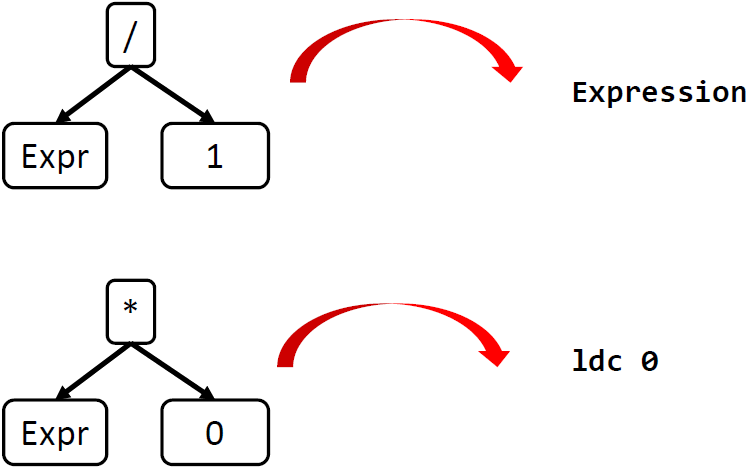
\includegraphics[width=0.5\linewidth]{alebra_vereinfachung.png}
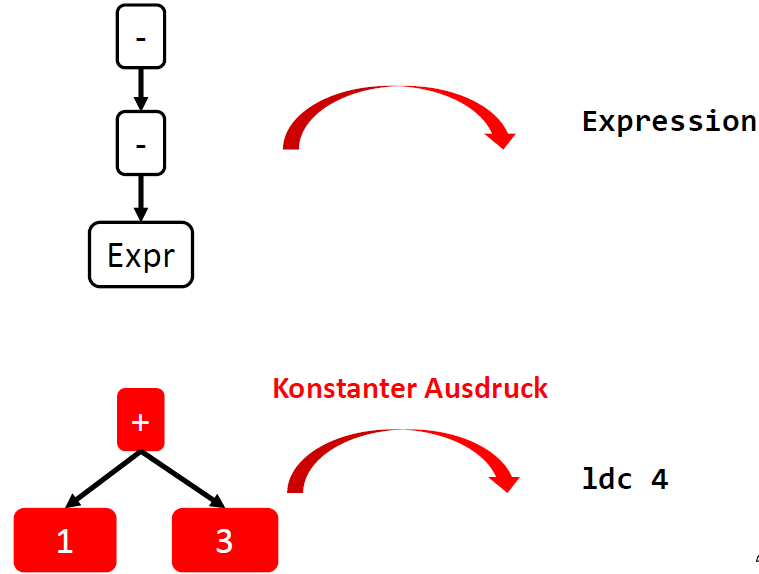
\includegraphics[width=0.5\linewidth]{alebra_vereinfachung2.png}

\subsection{Loop-Invariant Code}
\textbf{Invarianter Code aus der Schlaufe herausschieben}
\begin{lstlisting}
while (x < N * M) {
    k = y * M;
    x = x + k;
}
// Optimiert
k = y * M;
temp = N * M;
while (x < temp) {
    x = x + k;
}
\end{lstlisting}
\subsection{Common Subexpression Elimination}
\textbf{Wiederholt ausgewertete Teilausdrücke}
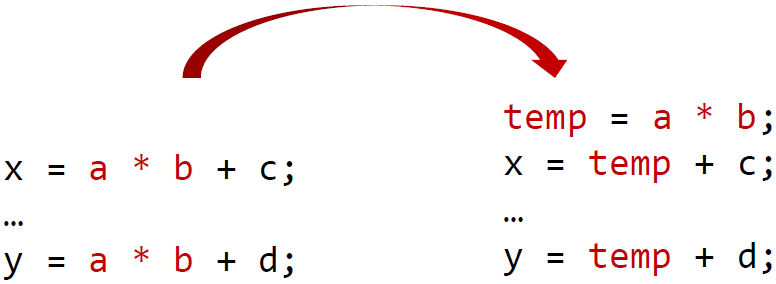
\includegraphics[width=0.5\linewidth]{subexpr_elimination.png}

\subsection{Dead Code}
\begin{lstlisting}
a = readInt();
b = a + 1;
writeInt(a);
c = b / 2; // Kein Lesen von c: Dead Code
\end{lstlisting}
\subsubsection{Elimination}
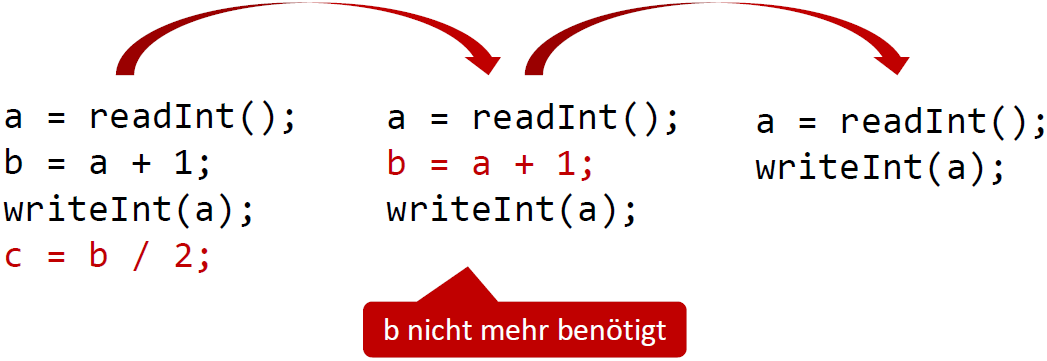
\includegraphics[width=0.5\linewidth]{dead_code.png}

\subsection{Redundatnes Lesen und Schreiben (Copy Propagation)}
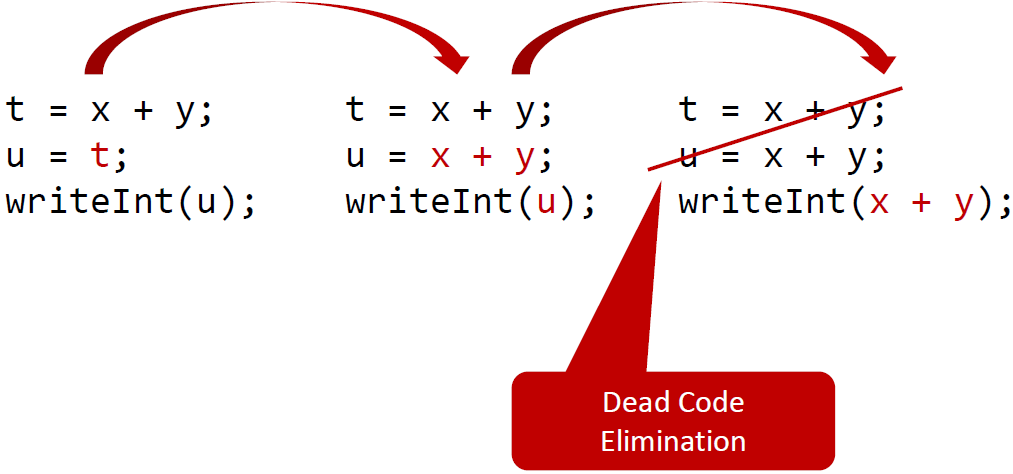
\includegraphics[width=0.5\linewidth]{copy_propagation.png}

\subsection{Constant Propagation (Constant Folding)}
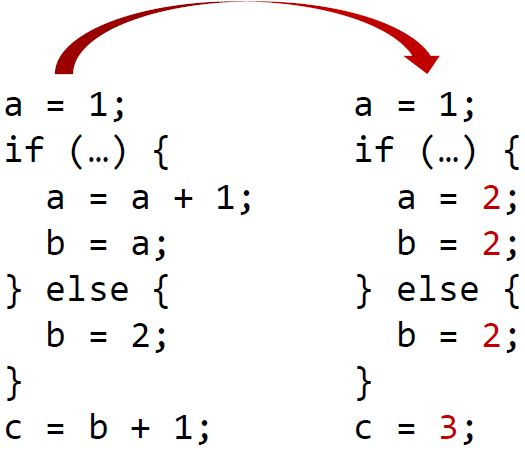
\includegraphics[width=0.3\linewidth]{constant_propagation.png}\\
\textbf{Danach kann Dead Code oder Duplikate entfernt werden}

\subsection{Partial Redundancy}
\textbf{Beim if-Pfad wird x + 4 zweimal evaluiert}\\
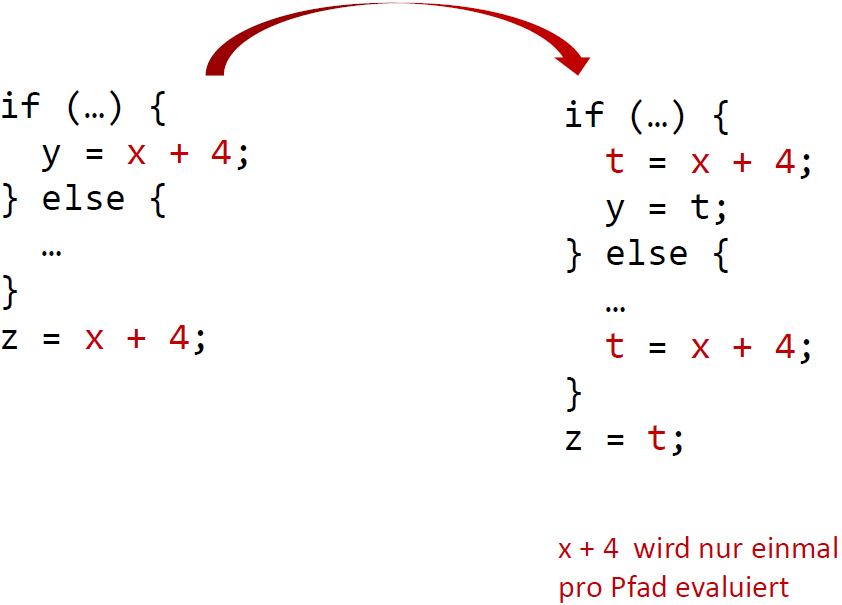
\includegraphics[width=0.5\linewidth]{partial_redundancy.png}

\subsection{Erkennung von Optimierungspotential}
\subsubsection{Static single Assignment}
Code-Transformation für einfachere Analyse \& Optimierung
\begin{itemize}
    \item Jede Variable wird nur einmal im Code zugewiesen
\end{itemize}
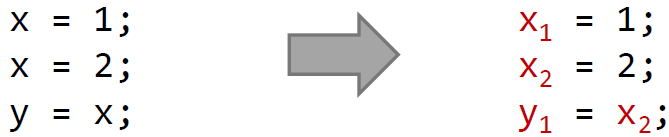
\includegraphics[width=0.4\linewidth]{ssa.png}\\ 
\textbf{Komplexer bei Verzweigungen}
\begin{itemize}
    \item Version von Variable nicht immer klar
    \item Phi Function: $\phi (x_1, x_2)$
    \begin{itemize}
        \item $x_1$ bei Pfad1
        \item $x_2$ bei Pfad2
    \end{itemize}
    \item Common Subexpressions werden mit SSA direkt entscheidbar
\end{itemize}
\textbf{SSA Berechnung}
\begin{itemize}
    \item Relativ kompliziert und teuer (besonders Phi)
    \item Günstigere Techniken gewünscht
\end{itemize}

 \subsubsection{Peephole Optimization}
 \begin{itemize}
     \item Optimierung für sehr kleine Anzahl Instruktionen
     \item In JIT-Compiler für Intermediate Code oder Maschinencode benutzt
     \item \textbf{Wende Optimierungsmuster auf Sliding Window an (z.B. 3 Operationen)}
 \end{itemize}
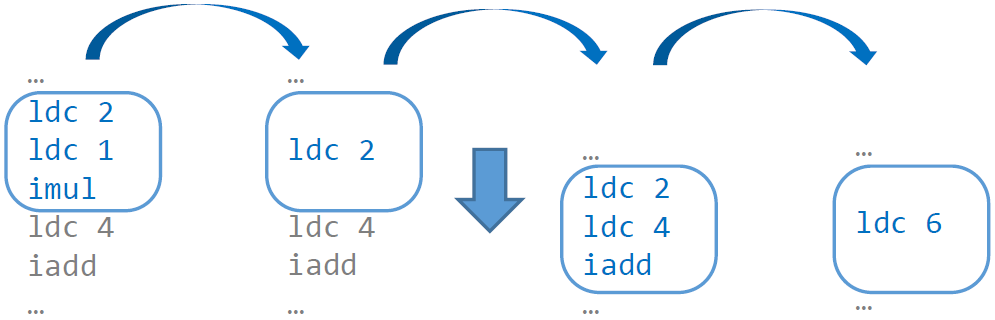
\includegraphics[width=0.5\linewidth]{peephole.png}

\subsubsection{Dataflow Analysis}
\begin{itemize}
    \item Mächtige generische Code-Analyse-Technik
    \item Für viele Optimierungen nützlich
\end{itemize}

\subsection{Summary}
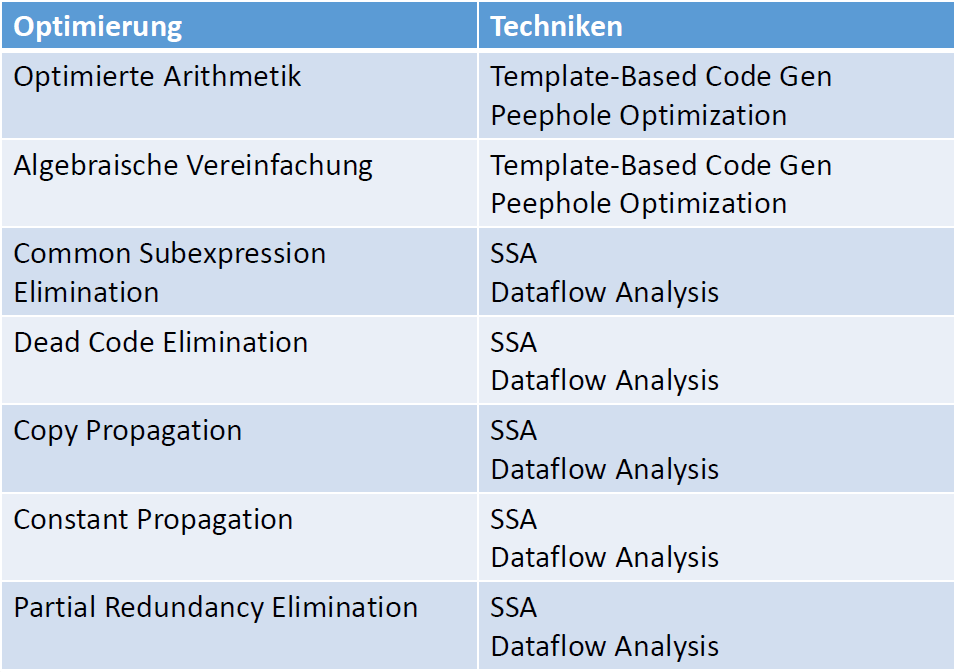
\includegraphics[width=0.5\linewidth]{summary.png}
